\chapter{Chapter 7: Logical Agents}

This chapter compiles high-scoring study notes and complete exam answers for \textbf{Unit VII: Logical Agents} of the OE-EC804A syllabus, adhering strictly to the \textbf{MAKAUT Answer Writing Guidelines}.


\section{Section 1: Propositional Logic Definitions and Tautology Proof (Q7.1)}

\subsection{1. Key Definitions in Propositional Logic}

\begin{itemize}
  \item   \textbf{Tautology:} A logical sentence that is true under every possible truth assignment of its variables. It represents a statement that is logically, necessarily true (e.g., $P \lor \neg P$).
  \item   \textbf{Contradiction (Unsatisfiable):} A logical sentence that is false under every possible truth assignment of its variables. It represents a statement that is logically impossible (e.g., $P \land \neg P$).
  \item   \textbf{Contingency:} A logical sentence that can be either true or false depending on the truth values assigned to its variables. Most everyday propositions are contingencies (e.g., $P \land Q$).
\end{itemize}


\subsection{2. Proof: $(((P \rightarrow Q) \rightarrow P) \rightarrow P)$ is a Tautology}
This formula is known as \textbf{Peirce's Law}. We construct a truth table to evaluate its truth value across all possible combinations of $P$ and $Q$.

\begin{table}[H]
\centering
\begin{tabular}{|p{\dimexpr 0.16666666666666666\textwidth - 2\tabcolsep - 1.5\arrayrulewidth\relax}|p{\dimexpr 0.16666666666666666\textwidth - 2\tabcolsep - 1.5\arrayrulewidth\relax}|p{\dimexpr 0.16666666666666666\textwidth - 2\tabcolsep - 1.5\arrayrulewidth\relax}|p{\dimexpr 0.16666666666666666\textwidth - 2\tabcolsep - 1.5\arrayrulewidth\relax}|p{\dimexpr 0.16666666666666666\textwidth - 2\tabcolsep - 1.5\arrayrulewidth\relax}|p{\dimexpr 0.16666666666666666\textwidth - 2\tabcolsep - 1.5\arrayrulewidth\relax}|}
\hline
Row & $P$ & $Q$ & $P \rightarrow Q$ & $(P \rightarrow Q) \rightarrow P$ & $((P \rightarrow Q) \rightarrow P) \rightarrow P$ \\
\hline
\textbf{1} & T & T & T & T & \textbf{T} \\
\hline
\textbf{2} & T & F & F & T & \textbf{T} \\
\hline
\textbf{3} & F & T & T & F & \textbf{T} \\
\hline
\textbf{4} & F & F & T & F & \textbf{T} \\
\hline
\end{tabular}
\end{table}

\subsubsection{Explanation of Steps:}
\textit{   }Column 4 ($P \rightarrow Q$):* False only when $P$ is True and $Q$ is False (Row 2).
\textit{   }Column 5 ($(P \rightarrow Q) \rightarrow P$):* Implication is false only if the premise ($(P \rightarrow Q)$) is True and the conclusion ($P$) is False. This happens in Row 3 (T $\rightarrow$ F) and Row 4 (T $\rightarrow$ F).
\textit{   }Column 6 ($((P \rightarrow Q) \rightarrow P) \rightarrow P$):* Implication is false only if Column 5 is True and $P$ is False. Let's verify:
\begin{itemize}
  \item   Row 1: T $\rightarrow$ T $\Rightarrow$ True.
  \item   Row 2: T $\rightarrow$ T $\Rightarrow$ True.
  \item   Row 3: F $\rightarrow$ F $\Rightarrow$ True.
  \item   Row 4: F $\rightarrow$ F $\Rightarrow$ True.
\end{itemize}

\textbf{Conclusion:} Since the final column is True in all possible rows, the sentence $(((P \rightarrow Q) \rightarrow P) \rightarrow P)$ is proved to be a \textbf{Tautology}. $\blacksquare$


\section{Section 2: Logical Inference Rules (Q7.2)}

Inference rules are patterns of logical deduction that derive a conclusion from premises.

\subsection{1. Modus Ponens}
\begin{itemize}
  \item   \textbf{Syntax:}
\end{itemize}
    \[ \frac{P, \quad P \rightarrow Q}{Q} \]
\begin{itemize}
  \item   \textbf{Description:} If both $P$ and "If $P$ then $Q$" are true, then $Q$ must be true.
  \item   \textbf{Truth Table Validation:}
  \item   We show that the sentence $((P \land (P \rightarrow Q)) \rightarrow Q)$ is a Tautology.
\end{itemize}

\begin{table}[H]
\centering
\begin{tabular}{|p{\dimexpr 0.16\textwidth - 2\tabcolsep - 1.5\arrayrulewidth\relax}|p{\dimexpr 0.21\textwidth - 2\tabcolsep - 1.5\arrayrulewidth\relax}|p{\dimexpr 0.21\textwidth - 2\tabcolsep - 1.5\arrayrulewidth\relax}|p{\dimexpr 0.21\textwidth - 2\tabcolsep - 1.5\arrayrulewidth\relax}|p{\dimexpr 0.21\textwidth - 2\tabcolsep - 1.5\arrayrulewidth\relax}|}
\hline
$P$ & $Q$ & $P \rightarrow Q$ & $P \land (P \rightarrow Q)$ & $(P \land (P \rightarrow Q)) \rightarrow Q$ \\
\hline
T & T & T & T & \textbf{T} \\
\hline
T & F & F & F & \textbf{T} \\
\hline
F & T & T & F & \textbf{T} \\
\hline
F & F & T & F & \textbf{T} \\
\hline
\end{tabular}
\end{table}


\subsection{2. Modus Tollens}
\begin{itemize}
  \item   \textbf{Syntax:}
\end{itemize}
    \[ \frac{\neg Q, \quad P \rightarrow Q}{\neg P} \]
\begin{itemize}
  \item   \textbf{Description:} If $P$ implies $Q$, and $Q$ is false, then $P$ must be false.
  \item   \textbf{Truth Table Validation:}
  \item   We show that the sentence $((\neg Q \land (P \rightarrow Q)) \rightarrow \neg P)$ is a Tautology.
\end{itemize}

\begin{table}[H]
\centering
\begin{tabular}{|p{\dimexpr 0.14285714285714285\textwidth - 2\tabcolsep - 1.5\arrayrulewidth\relax}|p{\dimexpr 0.14285714285714285\textwidth - 2\tabcolsep - 1.5\arrayrulewidth\relax}|p{\dimexpr 0.14285714285714285\textwidth - 2\tabcolsep - 1.5\arrayrulewidth\relax}|p{\dimexpr 0.14285714285714285\textwidth - 2\tabcolsep - 1.5\arrayrulewidth\relax}|p{\dimexpr 0.14285714285714285\textwidth - 2\tabcolsep - 1.5\arrayrulewidth\relax}|p{\dimexpr 0.14285714285714285\textwidth - 2\tabcolsep - 1.5\arrayrulewidth\relax}|p{\dimexpr 0.14285714285714285\textwidth - 2\tabcolsep - 1.5\arrayrulewidth\relax}|}
\hline
$P$ & $Q$ & $\neg P$ & $\neg Q$ & $P \rightarrow Q$ & $\neg Q \land (P \rightarrow Q)$ & $(\neg Q \land (P \rightarrow Q)) \rightarrow \neg P$ \\
\hline
T & T & F & F & T & F & \textbf{T} \\
\hline
T & F & F & T & F & F & \textbf{T} \\
\hline
F & T & T & F & T & F & \textbf{T} \\
\hline
F & F & T & T & T & T & \textbf{T} \\
\hline
\end{tabular}
\end{table}


\subsection{3. Resolution Rule}
\begin{itemize}
  \item   \textbf{Syntax:}
\end{itemize}
    \[ \frac{P \lor Q, \quad \neg P \lor R}{Q \lor R} \]
\begin{itemize}
  \item   \textbf{Description:} If we know that $P$ or $Q$ is true, and we also know that either $\neg P$ or $R$ is true, then we can resolve the conflict to conclude that $Q$ or $R$ must be true.
  \item   \textbf{Unit Resolution (Special Case where $R$ is empty):}
\end{itemize}
    \[ \frac{P \lor Q, \quad \neg P}{Q} \]


\section{Section 3: Knowledge-Based Agents and Wumpus World (Q7.3)}

\subsection{1. Knowledge-Based Agents}
A \textbf{Knowledge-Based Agent} is an agent whose internal state is defined by a \textbf{Knowledge Base (KB)} -- a set of representations of facts (sentences) about the world expressed in a formal logic language.

The agent interacts with its KB using two main functions:
\begin{itemize}
  \item   \textbf{`TELL`:} Adds a new sentence (percept information or inferred fact) to the knowledge base.
  \item   \textbf{`ASK`:} Queries the knowledge base to determine what action should be taken next.
\end{itemize}

\subsubsection{The KB-Agent Working Loop:}
\begin{lstlisting}
function KB-AGENT(percept) returns an action
  persistent: KB, a knowledge base
              t, a counter, initially 0

  TELL(KB, MAKE-PERCEPT-SENTENCE(percept, t))
  action <- ASK(KB, MAKE-ACTION-QUERY(t))
  TELL(KB, MAKE-ACTION-SENTENCE(action, t))
  t <- t + 1
  return action
\end{lstlisting}


\subsection{2. The Wumpus World Environment}
The \textbf{Wumpus World} is a grid environment used to demonstrate logical reasoning. An agent must navigate the grid to find a heap of gold and return safely without falling into a pit or being eaten by the beast (the Wumpus).

\begin{figure}[H]
\centering
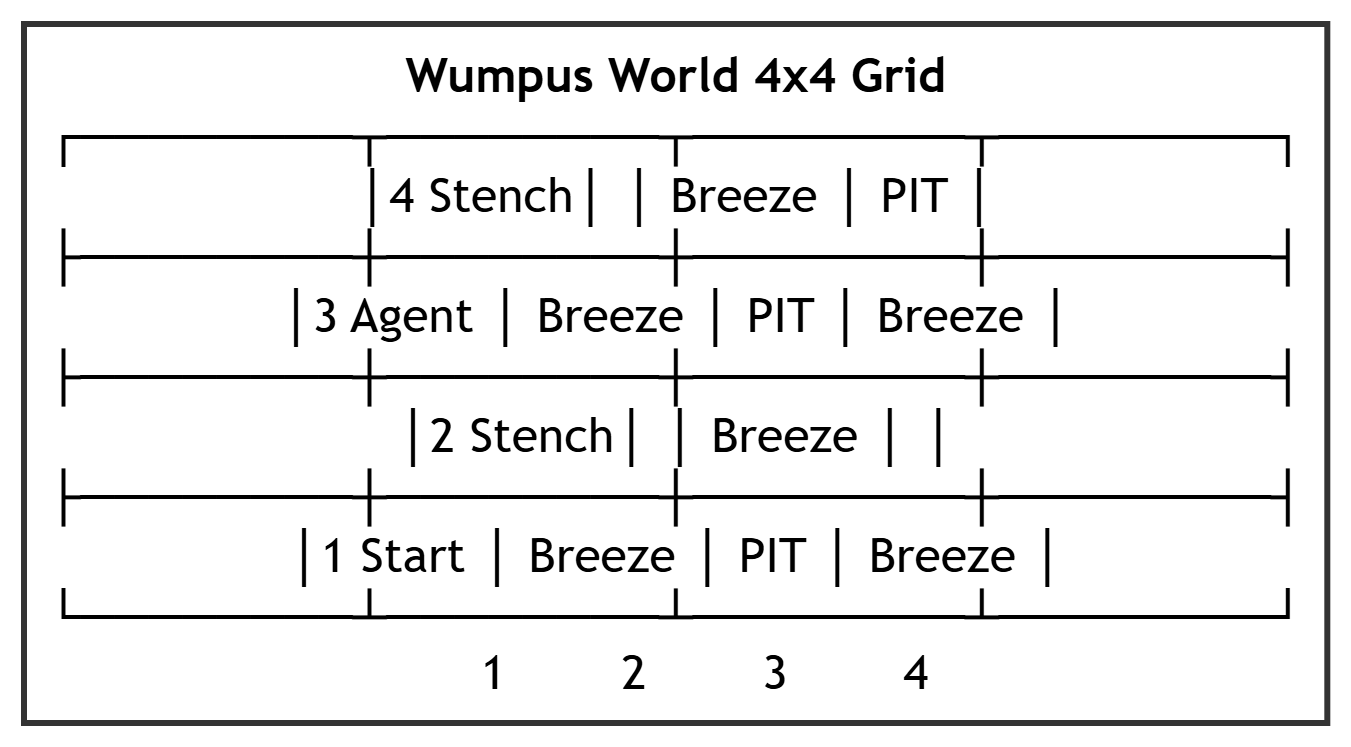
\includegraphics[width=0.75\textwidth,height=0.32\textheight,keepaspectratio]{../Images/chapter_07/wumpus_world_grid.png}
\caption{Wumpus World Grid Layout}
\end{figure}

\subsubsection{PEAS Description of Wumpus World:}
\begin{itemize}
  \item   \textbf{P (Performance):} $+1000$ for climbing out of the cave with gold; $-1000$ for falling into a pit or being eaten; $-1$ for each action taken; $-10$ for using the arrow.
  \item   \textbf{E (Environment):} $4 \times 4$ grid of rooms. Pits are placed randomly (each cell has $0.2$ probability of containing a pit). The Wumpus is in a single random cell. Gold is in a single random cell.
  \item   \textbf{A (Actuators):} Turn Left, Turn Right, Forward, Grab (gold), Shoot (arrow), Climb (out).
  \item   \textbf{S (Sensors):}
\end{itemize}
    \textit{   }Stench:* Felt in cells adjacent to the Wumpus.
    \textit{   }Breeze:* Felt in cells adjacent to pits.
    \textit{   }Glitter:* Felt in the cell containing the gold.
    \textit{   }Bump:* Felt when walking into a wall.
    \textit{   }Scream:* Heard anywhere in the cave when the Wumpus is killed.


\subsection{3. Step-by-Step Safe Logic Reasoning Example}
Let the agent start at cell $(1,1)$. Let's trace how the agent reasons using logic rules to move safely:

\begin{enumerate}
  \item \textbf{Initial Percept at $(1,1)$:} `[None, None, None, None, None]` (No Stench, No Breeze).
\end{enumerate}
    \textit{   }Logical Rule:* If there is no Breeze at $(1,1)$, then there is no pit in $(1,2)$ and $(2,1)$.
    \textit{   }Logical Rule:* If there is no Stench at $(1,1)$, then the Wumpus is not in $(1,2)$ or $(2,1)$.
    \textit{   }Deduction:* Cells \textbf{$(1,2)$} and \textbf{$(2,1)$} are safe.
\begin{enumerate}
  \item \textbf{Move to $(2,1)$:}
\end{enumerate}
    \textit{   }Percept at $(2,1)$:* `[None, Breeze, None, None, None]` (Breeze detected).
    \textit{   }Logical Rule:* A Breeze at $(2,1)$ implies a pit exists in one of the adjacent cells: $(1,1)$, $(2,2)$, or $(3,1)$.
    \textit{   }Deduction:* Since $(1,1)$ is the start and is safe, the pit is either in $(2,2)$ or $(3,1)$. The agent cannot determine which one is the pit yet, so it backtracks.
\begin{enumerate}
  \item \textbf{Return to $(1,1)$ and move to $(1,2)$:}
\end{enumerate}
    \textit{   }Percept at $(1,2)$:* `[Stench, None, None, None, None]` (Stench detected, No Breeze).
    \textit{   }Logical Rule:* Since there is no Breeze at $(1,2)$, adjacent cells $(1,3)$ and $(2,2)$ have no pits.
    \textit{   }Deduction:*
\begin{itemize}
  \item   Since $(2,2)$ has no pit, the pit detected from $(2,1)$ must be in \textbf{$(3,1)$}.
  \item   A Stench at $(1,2)$ implies the Wumpus is in $(1,1)$, $(1,3)$, or $(2,2)$.
  \item   Since $(1,1)$ is safe, and $(2,2)$ has no Stench (verified earlier from \$1,1\$), the Wumpus must be in \textbf{$(1,3)$}.
\end{itemize}
    \textit{   }Resulting Safe Plan:* Cell \textbf{$(2,2)$} is free of both pits and Wumpus, and is safe to enter next.
